\documentclass{article}

\usepackage[top=2.5cm,left=2.5cm,right=2.5cm,bottom=2.5cm]{geometry}
\usepackage[utf8]{inputenc}
\usepackage[T1]{fontenc}
\usepackage[french]{babel}
\usepackage{graphicx}
\usepackage{multicol}
\usepackage{pdflscape}
\usepackage[pdfborder={0 0 0}]{hyperref}

\title{
\includegraphics{img/logo.png}\vspace{2cm}\\
    Stage chez Let There Be Light \\
    \large Rapport de stage Exia A4}

\date{24 Mars 2018}

\author{Stagiaire : Baptiste \bsc{Saclier} \\
    Maître de stage : Benjamin \bsc{Petit}\\
    Pilote de formation : Julio \bsc{Santilario}}

\begin{document}

    \maketitle

    \clearpage

    \tableofcontents

    \section{Introduction}

    Dans le cadre de ma 3\up{e} année au CESI EXiA, j'éfféctue actuellement un stage chez Let There Be Light.
    Cette entreprise réalise des dispositifs interactifs pour l'événementiel, la communication et la culture.

    Ce rapport relate de cette entreprise et des projets sur lesquels j'ai travaillé.

    \clearpage

    \section{Let There Be Light}

La société Let There Be Light (ou LTBL) est une société qui réalise des dispositifs interactifs pour l'événementiel, la communication et la culture.
Elle fut fondée en 2014 par Benjamin \bsc{Petit} et Antoine \bsc{Vanel} sous le nom de Beam'Art.
En 2016, elle change de nom et de statut pour devenir l'entreprise que l'on connaît aujourd'hui.
Actuellement, M. \bsc{Petit} en est le seul dirigeant et emploi 2 personnes.

\begin{description}
    \item[2012] Première fête des Lumières de Lyon dans le cadre d'une association avec un spectacle interactif nommé "Hypermétrope"
    \item[2014] Fondation de la société Beam'Art
    \item[2014] Installation interactive "Hi Striker" sur le palais de justice
    \item[2014] Mapping "TranJS" à Bernes
    \item[2015] Installation interactive "Lumibus" pour Keolis
    \item[2016] Changement de nom pour devenir Let There Be Light
    \item[2016] Participation à la création du showroom Pavillon de l'innovation pour Michelin
    \item[2017] Scénographie au Transbordeurs "DELete"
\end{description}

\subsection{Structure}

Let There Be Light est un partenaire de la société Vendredi 4.
Vendredi 4 est une société de communication spécialisée dans l'interaction.
Les contrats sont obtenus par Sylvie \bsc{Madamour}, la charte graphique du projet est alors composée par Vendredi 4.
LTBL intervient sur l'intégration de cette charte graphique dans les installations interactives dans des salons ou des showrooms.

Les équipes de Vendredi 4 et de LTBL sont assez réduites.
L'effectif de Vendredi 4 est de 3 employé quand LTBL compte un unique employé (Benjamin \bsc{Petit}) et deux consultants : Corentin \bsc{Limoge} et Alexander \bsc{Feller}.

\begin{figure}[h]
    \centering
    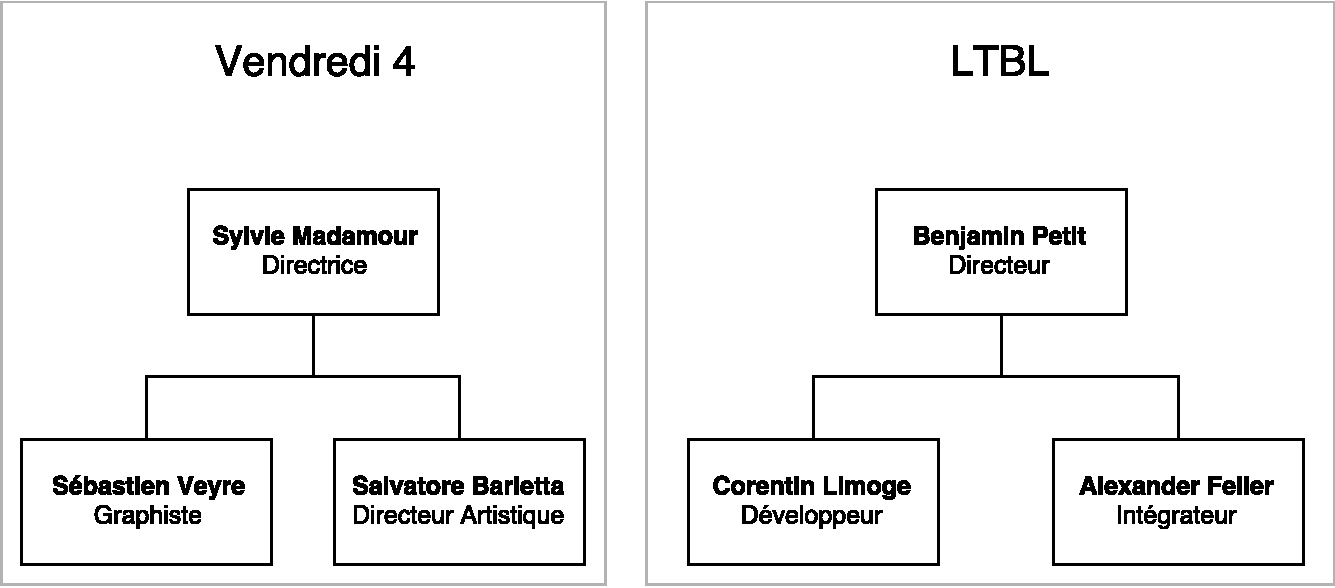
\includegraphics[scale=0.7]{img/Structure-LTBL.pdf}
    \caption{Structure de LTBL et Vendredi 4}
\end{figure}

Les deux entreprises sont très liées, elles partagent les mêmes locaux et communiquent beaucoup ensemble sur les projets en cours et à venir.

On retrouve alors Benjamin \bsc{Petit}, le gérant, et Corentin \bsc{Limoge} du côté LTBL.
Benjamin s'occupe des conseils et de la gestion de l'entreprise.
Il s'occupe aussi de l'aspect technique des installations par le choix des technologies de pointage et d'affichage.
Corentin est employé par LTBL, mais dispose d'un statut d'auto-entrepreneur, on peut alors le considérer comme un consultant.
Corentin est en charge du développement des applications qui seront exécutées sur les installations.

Du côté Vendredi 4, on retrouve Sylvie \bsc{Madamour}, la directrice, Salvatore \bsc{Barletta}, directeur artistique, et Sébastien \bsc{Veyre}, graphiste.
Sylvie est en charge des contrats, devis et de la communication avec les clients.
Salvatore est directeur artistique chez Vendredi 4, il s'occupe de concevoir et présenter les design des installations aux clients.
Sébastien est graphiste et est en charge de représenter les futures interfaces des installations, mais aussi de travailler sur des rendus en Motion Design\footnote{Une technique d'animation graphique ayant pour but de mettre en valeur le mouvement et l'animation.} Pour donner un premier aperçu de la future application pour les clients et les intégrateurs.

\subsection{Projets}

Les deux entreprises travaillent ensemble pour proposer des services suivants :

\begin{itemize}
    \item Conseils techniques
    \item Conseils en interaction
    \item Design graphique
    \item Développement d'applications interactives
    \item Installations
\end{itemize}

Ainsi, les deux entreprises peuvent suivre la production d'une application interactive de sa conception jusqu'à son installation.

\medskip

Les projets suivis par LTBL sont les suivants :

\paragraph{Dispositifs de présentation interactifs} le plus souvent utilisés dans les salons et showrooms, les dispositifs interactifs permettent une présentation des produits de manière esthétique.
L'objectif de LTBL est donc de concevoir cette installation.
Cela passe par la conception du système physique est des composants requis mais aussi par la conception et le développement de l'interface utilisateur qui doit être réactive et esthétique.
La majorité de ce type de projet est la présentation d'informations sur un produit sur un écran tactile

\paragraph{Vidéo Mapping} Le plus souvent présenté lors d'événements, le vidéo mapping consiste en la projection d'une image déformée sur une structure pouvant être un bâtiment ou une installation spécifique.
Cette image utilise une représentation de la structure pour se déformer et épouser sa forme lors de la projection.
Ce type d'installation permet, au travers de jeux de lumière et d'illusions, de donner vie à la structure ou au bâtiment.
On retrouve ce type d'installation à la fête des Lumières de Lyon par exemple.

\paragraph{Conseils techniques ou en interaction} Fort de son expérience dans le domaine de l'interactivité, LTBL peut aussi donner des conseils en interactivité dans le cadre de projets cités plus haut.

\paragraph{Fête des Lumières} La fête des Lumières est une manifestation Lyonnaise prenant place aux endroits importants de la ville.
Cette fête met en lumière de nombreuses installations lumineuses et interactives.
Chaque année, LTBL peut proposer un projet d'installation en rapport avec un bâtiment de la ville sur lequel s'installer.
Ce projet est alors évalué et est accepté ou non en fonction de la faisabilité, l'esthétique et le coût de l'installation.
La dernière fête des Lumières à laquelle a participé LTBL fut celle de 2015 avec une installation nommée "Lumibus".
Cette installation présentait un Bus muni de panneaux LED réagissant aux accélérations et freinages de celui-ci.
Les années précédentes, LTBL a aussi présenté Hi Striker, une installation reprenant le jeu de foire de la massue où les participants doivent taper le plus fort possible sur un capteur à l'aide d'une massue.
Plus la frappe est forte plus le bâtiment s'illumine.
Cette installation se trouvait au palais de justice.
Plus récemment, LTBL a participé à la fête des Lumières de Hong Kong avec un projet reprenant le même principe, mais en animant un dragon.

\begin{figure}[h]
    \centering
    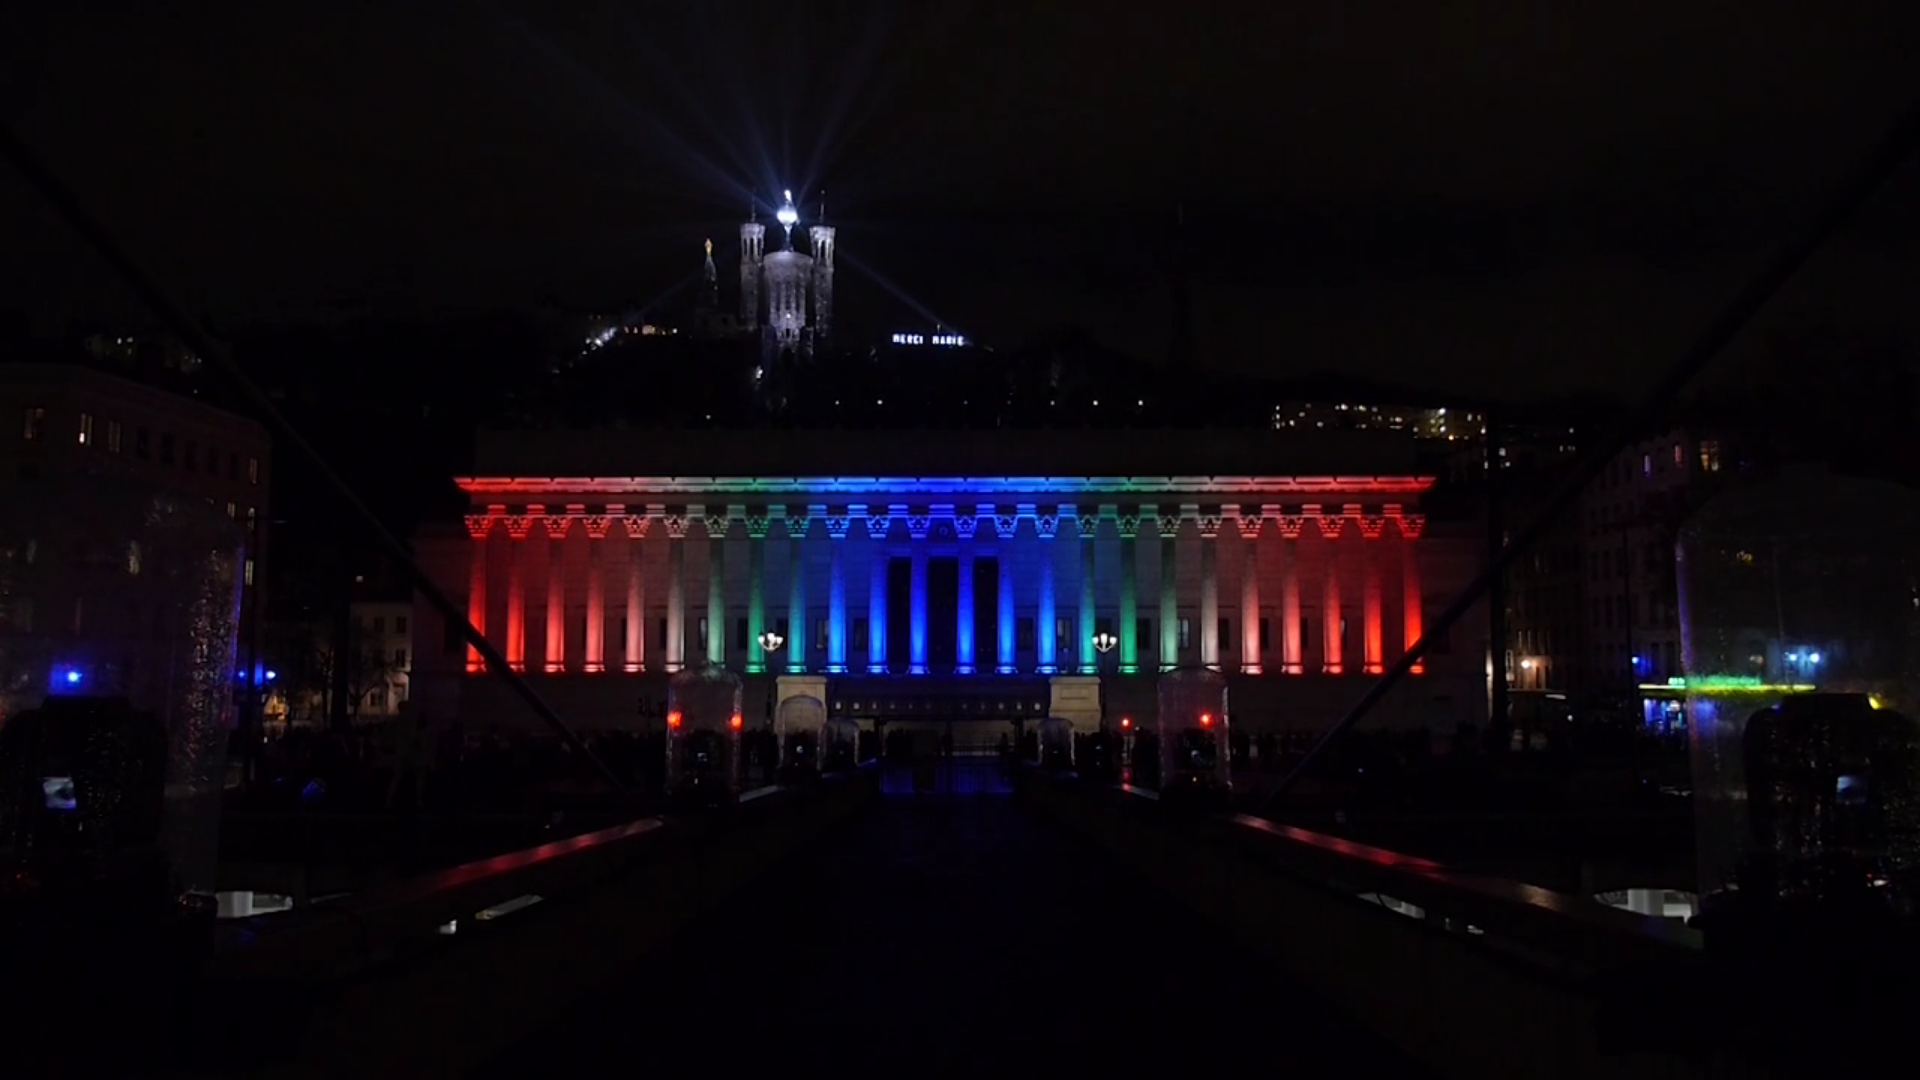
\includegraphics[scale=0.2]{img/hi-striker.png}
    \caption{L'installation "Hi Striker" à la fête des Lumières de Lyon}
\end{figure}


\begin{figure}[h]
    \centering
    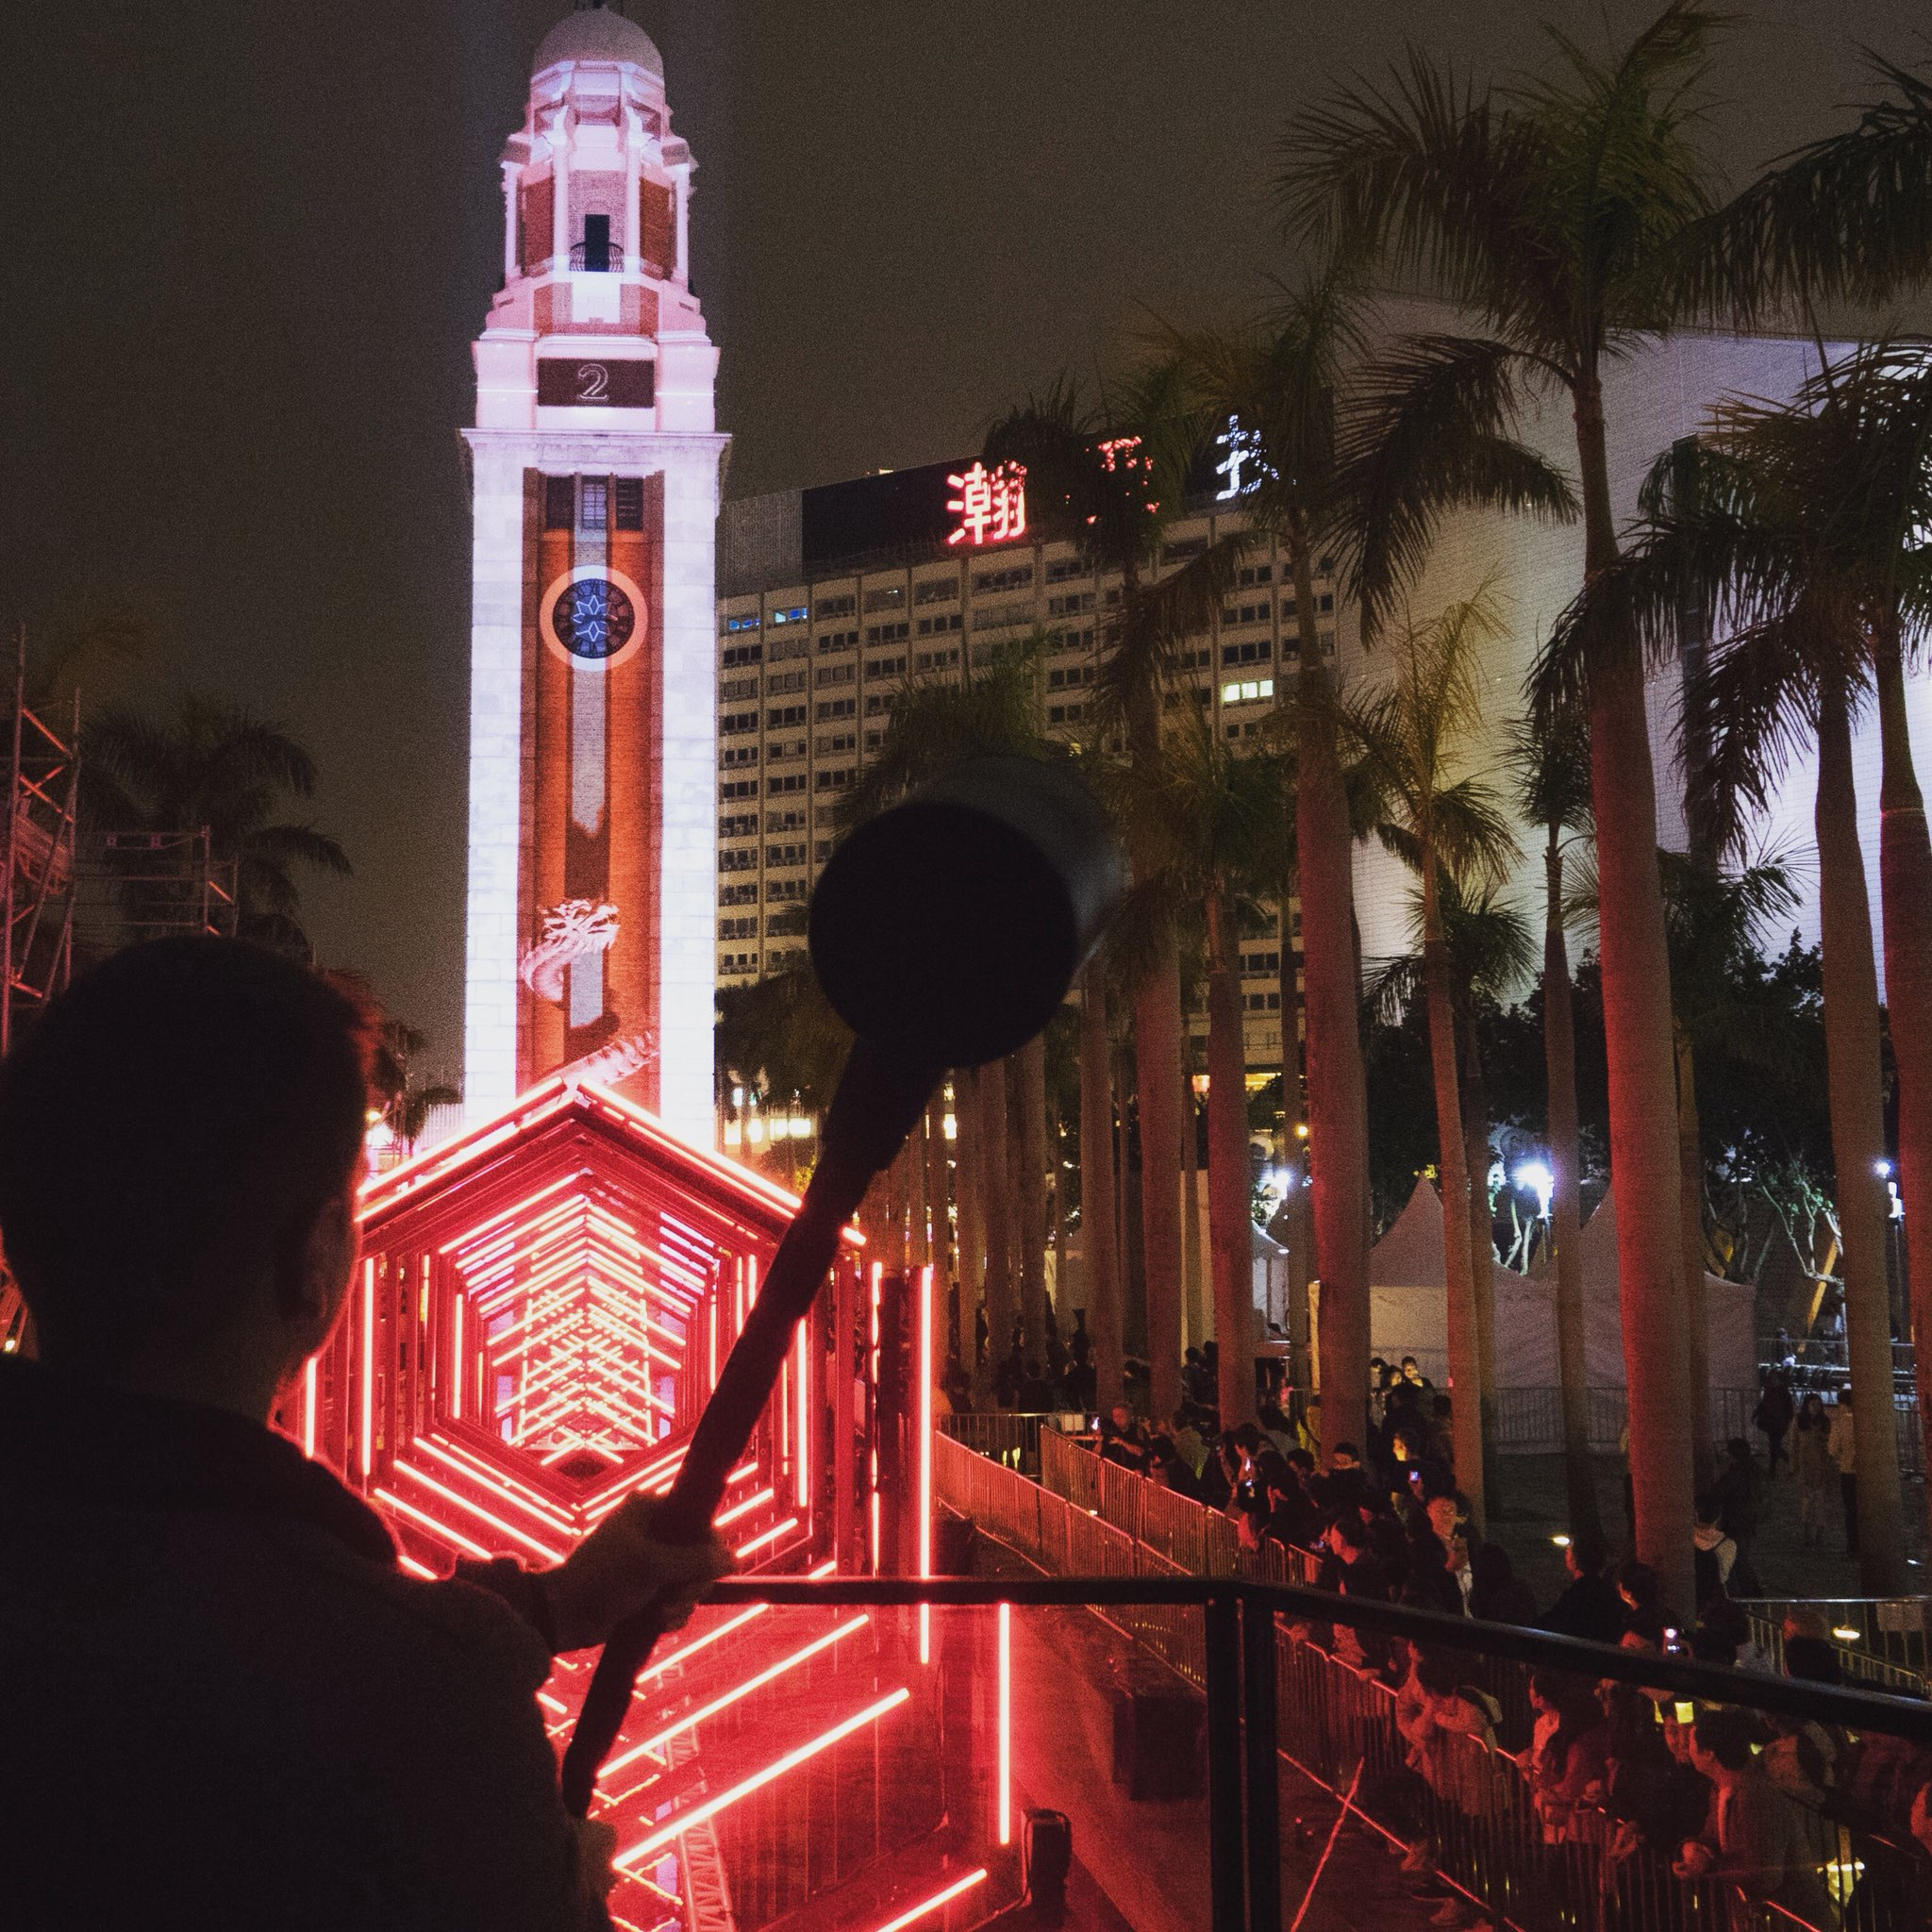
\includegraphics[scale=0.15]{img/long-striker.jpg}
    \caption{L'installation "Long Striker" à la fête des Lumières de Hong Kong}
\end{figure}

\clearpage

\subsubsection{Clients}

Les clients de LTBL et de Vendredi 4 sont, le plus souvent, de la région Rhône-Alpes, mais peuvent aussi être en région parisienne.
Ces clients sont des PME ou des grands groupes désirant de nouvelles installations interactives pour leurs showrooms.
Au travers de ces installations, ils peuvent montrer leur produit de manière esthétique à leurs clients.
Les showrooms ne sont pas les seuls installations organisées par LTBL, on retrouve aussi des présentations de produits pour les salons ou l'affichage de données pour la productivité.

\bigskip

Quelques clients :

\begin{multicols}{2}
    \begin{itemize}
        \item Biomérieux
        \item EDF
        \item Michelin
        \item Somfy
        \item Visiativ
        \item Courchevel
        \item Fête des Lumières
        \item Et bien d'autres \ldots
    \end{itemize}
\end{multicols}

    \subsection{bioMérieux}

BioMérieux est une entreprise spécialisée dans le diagnostic in vitro et dans la microbiologie.
Cette entreprice concoit et fabrique des instruments permettant de diagnostiquer des maladies et de faire des analyses microbiologiques.

BioMérieux dispose d'un showroom permettant de montrer leur produits à leurs futurs clients.
Dans ce Showroom, un ensemble de dispositifs interactifs sont mis en place pour presenter les produits et l'entreprise.
Parmis ces équipement, on retrouve l'espace solution.
Cet espace présente un exemplaire physique des principales machines concus par bioMérieux.
Un projecteur permet alors d'afficher une image sur une vitre opacifiante.
On utilise alors une application pour montrer 

    \section{Blind Test \aha}

\subsection{\ah Arena}

\ah est le premier gérant d'hôtel de France et le 6e mondial.
À l'occasion d'un partenariat, le Palais omnisports de Paris-Bercy s'est vu renommé \aha pour 10 ans.

Le site accueillant beaucoup de concerts et de spectateurs, Accorshotel a voulu communiquer au travers d'une installation interactive.
Cette installation est un blind test composé d'un écran et d'un iPad permettant de saisir les réponses.

Le jeu est simple : une chanson est jouée sur l'écran et le titre de cette chanson est indiqué.
Le joueur dispose alors de 45 secondes pour trouver l'artiste en question parmi les 4 proposé.
On enchaîne ainsi sur 6 questions qui se terminent sur le résultat du jeu affiché à l'utilisateur.

\subsection{Technologies}

Les technologies utilisées dans ce projet sont standards et étaient déjà maîtrisées par les membres de l'équipe.
On retrouve alors une application \emph{Electron} pour l'affichage sur l'écran et un serveur NodeJS avec le framework \emph{Express} pour servir les fichiers et gérer le jeu.
Enfin, on utilise \emph{Socket.io} pour les WebSocket apportant de l'interactivité.

\subsubsection{Express}

Express est une librairie utilisant les capacités de NodeJs (inclus dans \emph{Electron}) à mettre en place un serveur Web.
Express permet de répondre à une URL, mais aussi de servir des fichiers en tout genre.

Nous avons choisi Express car il est léger et simple à mettre en place.
Il dispose d'une grande communauté et permet de mettre en place un serveur Web et websocket rapidement.

Nous n'avions pas besoin ici d'une solution plus lourde car les seules interactions HTTP sont les demandes de médias comme la musique et les images ou la demande de page WEB.
Le reste des interactions s'effectuent au travers des Websockets.

\subsubsection{WebSockets}

La technologie de Websocket est un protocole Web de connexion bidirectionnel.
Ils permettent au serveur et au client de conserver une connexion TCP bidirectionnelle.

Ainsi il est possible au client d'envoyer des paquets arbitraires au serveur, mais aussi au serveur d'envoyer des paquets au client à n'importe quel moment.
Ainsi, il est possible de rendre l'application très interactive et dynamique.

Nous avons utilisé les WebSockets pour toute la communication entre le serveur et les clients (Écran et iPad) avec l'aide de Socket.io.
Cette librairie se place comme une surcouche aux websocket et reprend l'aspect événementiel de Nodejs.
En effet, elle met à disposition du développeur un objet \texttt{socket} agissant comme un émetteur et un récepteur d'événements.
Chaque événement est composé d'un nom et d'un objet de contexte.
Lors de l'émission, l'objet \texttt{socket} transmet l'événement et le contexte au client connecté.
Il est aussi possible de recevoir des événements et ainsi de communiquer de manière bidirectionnelle.

\subsection{Structure}

Le Blind Test se compose de 3 éléments.

\paragraph{Le serveur Web} présent dans le processus principal de l'application Electron, il gère tout le jeu du début à la fin.
Il présente un serveur de fichiers permettant l'accès aux fichiers audio, aux fichiers d'image et aux pages Web depuis l'iPad et l'affichage.
Il dispose aussi d'un serveur WebSockets permettant une communication bidirectionnelle entre les clients (iPad et TV) et le serveur.

Ce serveur Web dispose d'un état définissant l'état actuel du jeu.
Cet état est transmis à tous les clients pour qu'ils actualisent leurs affichages lors d'un changement et de la connexion d'un nouveau client.

Le serveur Web construit en parallèle un objet Javascript \texttt{Game} contenant toutes les questions à poser, la question actuellement posée, les réponses des joueurs et le score.
Cet objet \texttt{Game} est transmis à chaque client lors de leur connexion ou lors du changement d'état du jeu.

Dès que l'état du jeu change, un événement socket.io est transmis à tous les clients connectés pour qu'ils actualisent leur affichage en fonction des données transmises par le serveur.

\paragraph{Les clients (TV et iPad)} Chacun charge une page HTML spécifique possédant un script spécifique.
Ce script va afficher le bon écran en fonction de l'état du jeu envoyé par le serveur et, éventuellement, demander une interaction à l'utilisateur.

Dès qu'un joueur tape sur une réponse, l'iPad envoie à son tour un paquet WebSocket au serveur pour qu'il l'enregistre et change d'état.
Le jeu continue alors jusqu'à ce que toutes les questions de tous les joueurs soient posées.

\begin{figure}[h]
    \centering
    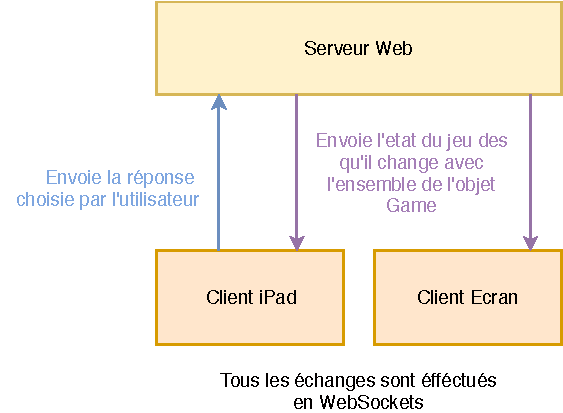
\includegraphics{img/ah-blindtest.pdf}
    \caption{Structure du jeu Blind Test}
\end{figure}

\subparagraph{TV} Coté TV, l'affichage est simple et permet d'afficher le score de l'utilisateur ainsi que de jouer la musique.
L'écran n'étant pas tactile, il ne permet que l'affichage d'informations sur l'état du jeu, mais aucune interactivité n'est possible directement.
Le client TV est une fenêtre de l'application Electron qui se connecte au serveur express pour charger l'interface.

\subparagraph{iPad} Coté iPad, une application de kiosque permet d'afficher une page Web sans autre élément d'interface.
Cette page Web est chargée depuis le serveur et propose des choix à l'utilisateur en fonction de l'état du jeu.
Cela peut être le nombre de joueurs, le nom de l'artiste en cours de lecture ou simplement une demande pour passer à la question suivante.

\subsubsection{Design}

Le design de l'application était fourni avec la demande du client et nous avons juste intégré ce design en extrayant des images clés du fichier Photoshop du designer.

\begin{figure}[h]
    \centering
    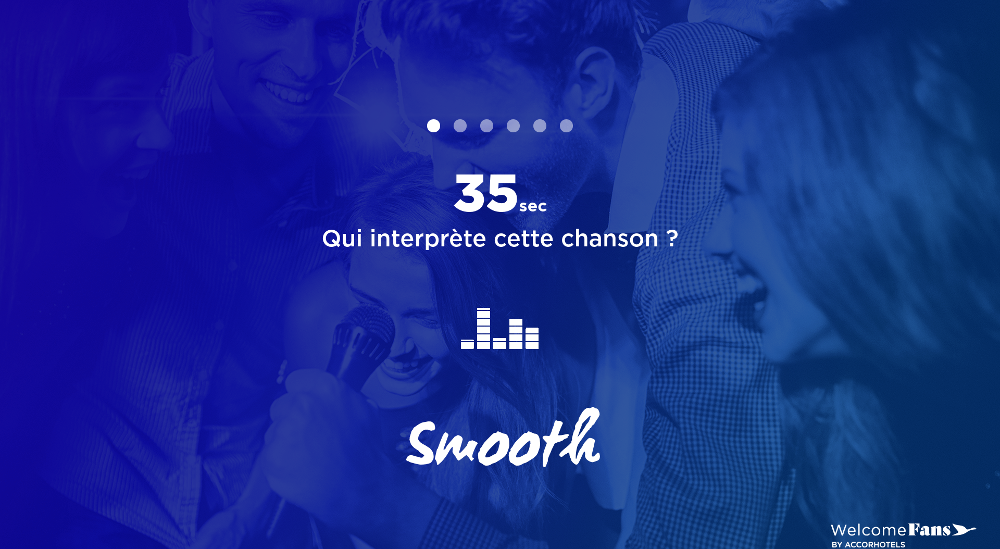
\includegraphics[scale=0.23]{img/blind-test-tv.png}
    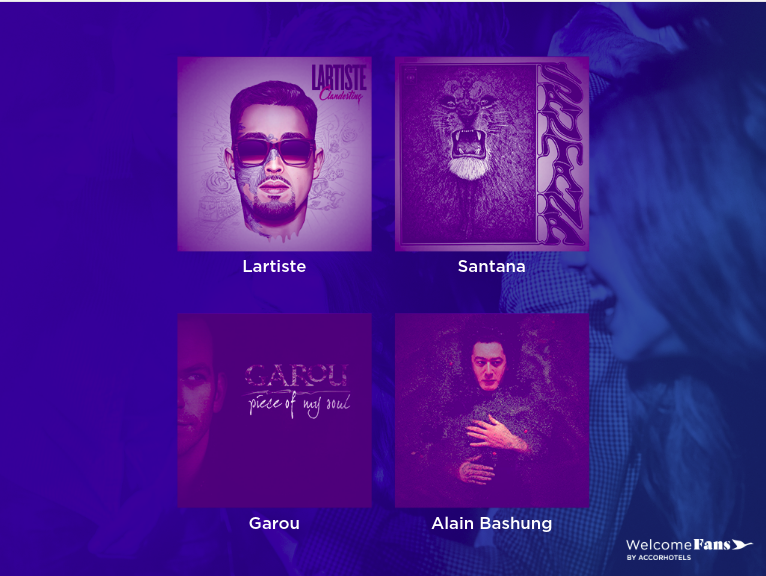
\includegraphics[scale=0.22]{img/blind-test-ipad.png}
    \caption{Une vue du Blind Test côté TV (à gauche) et côté iPad (à droite)}
\end{figure}

\subsubsection{Installation}

Je n'ai pas pu assister à l'installation du lundi 29 janvier, mais j'ai tout de même travaillé dessus à l'occasion de correction de bugs.

L'installation présente un grand écran connecté au serveur affichant l'interface TV sur une machine Windows hébergeant le serveur websocket que l'iPad pourra contacter.
On y retrouve bien évidemment L'iPad verrouillé pour éviter de sortir de l'application.
Ces deux terminaux sont connectés à une même borne WiFi permettant de disposer de son propre réseau évitant ainsi les latences dues à une éventuelle surcharge du réseau environnant.
Cette borne WiFi fait office de routeur vers l'extérieur, mais aussi de serveur DHCP et de point d'accès WiFi.

\begin{figure}[h]
    \centering
    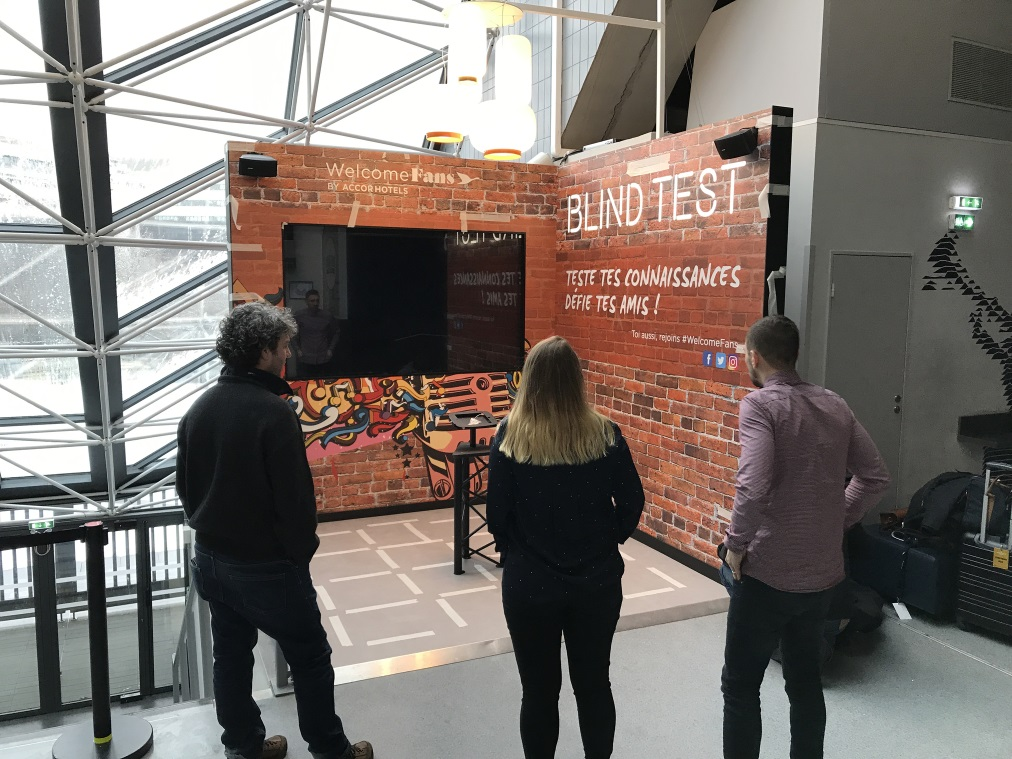
\includegraphics[scale=0.4]{img/accorhotel-blindtest-resize.jpg}
    \caption{Installation du Blind test au \aha}
\end{figure}

\subsubsection{Conclusion}

Ce projet fut intéressant et intense, car nous l'avons réalisé en seulement 2 jours.
Ce fut une bonne expérience de travail d'équipe et m'a permis de tester un projet à court délai.
Enfin, ce projet m'a permis de voir les techniques permettant de synchroniser l'état de multiples machines au travers de Websocket.


    \section{Bornes de présentation Somfy}

\subsection{Somfy}

Somfy est un entreprise concevant des systèmes domotiques à l'attention du grand public.
Dans une démarche de communication, Somfy a contacté LTBL pour la creation de 11 bornes interactives qui seront mises en place dans les magasins vendant les produits de la marque.

\subsection{Besoins}

L'objectif de ce projet est de concevoir et de produire 11 machines permettant d'afficher des informations sur l'entreprise et ses produits.
Ces informations peuvent être des vidéos, du texte ou des images.

Dans ce projet, je n'ai pas travaillé sur le développement de l'application de présentation mais sur la mise en place des 11 machines permettant son execution.
Ces 11 machines devaient presenter un système de visionnage pour réduire au maximum les possibilités de l'utilisateur.

\subsection{Recherches et choix du système}

Pour ce nouveau projet, j'ai proposé à mon maître de stage d'utiliser un système Linux pour l'execution des applications sur les bornes.
Cela a pour avantage une plus grande flexibilité et capacité de customisation mais aussi une gratuité de la license.
En effet, il est simple de mettre en place un système captif sur une machine linux car on contrôle chaque élément de l'OS .

Pour le système je me suis dirigé vers un membre de la famille Ubuntu pour sa stabilité et la grande communauté qui se forme autour.

J'ai alors découvert Ubuntu Core qui permet la creation de système embarqués et minimalistes.
Ubuntu Core est une varante de Ubuntu se basant sur des paquets unitaire séparés les uns des autres.
Cela permet de séparer chaque application et d'autoriser leur communication sur certains canaux particulier appelés interfaces.
Ce système rapelle beaucoup les systèmes mobiles comme Android ou IOS exigeant des permissions définies à l'avance pour que les applications aient acces à certaines fonctionnalités.
Ubuntu Core utilise Snapcraft, un gestionnaire de paquet permettant cette séparation des applications.
De pars sa complexitée et de l'abscense de serveur X sur snapcraft, je n'ai pas retenu cette solution et me suis penché sur Ubuntu Server.

Ubuntu Server est une version de Ubuntu sans les composants de bureau classique.
Il permet de composer son propre système sans la lourdeur des applications graphiques inutiles dans le contexte des bornes Somfy.
J'ai donc choisi cette distribution ayant pour objectif d'installer un environnement de bureau manuellement.

\subsection{Environnement de kiosk}

Pour mettre en place l'environnement d'affichage, j'ai commencé par installer le serveur X .
Le serveur X est le logiciel en charge d'afficher l'interface à l'utilisateur au travers d'un protocol spécifique.

Apres avoir installé ce logiciel, il faut installer un système de gestion de fenètres qui sera en charge d'afficher les différentes fenêtre à la bonne taille et dans le bon contexte.
Pour le gestionnaire de fenêtres, j'ai choisi xfce car il est légé et propose beaucoup de fonctionnalités.
Le gestionnaire de fenêtre est essentiel car il permet aux applications de correctement se dimentionner et de passer en plein ecran pour empècher l'utilisateur d'éfféctuer des actions non désirées.

Enfin, on peut installer notre application et la démarrer.

Il faut bien sur automatiser tout cela pour que l'ensemble puisse se démarrer automatiquement en même temps que la machine pour éviter tout action manuelle de l'installateur.
Pour ce faire j'ai été amené a modifier le pipeline de démarrage du système.
Tout d'abord il faut créer un nouvel utilisateur qui sera en charge d'executer l'application pour eviter qu'elle ne soit éxécuté en tant qu'administrateur.
Ensuite, il faut modifier le comportement de connexion sur la première console pour qu'elle se connecte automatiquement avec l'utilisateur en charge de l'execution du programme.
L'utilisateur connecté, on execute le script de démarrage qui se charge de démarrer le serveur X, le gestionnaire de fenêtres et l'application.

Nous disposons alors d'un système de kiosk fonctionnel et sécurisé.

\subsection{Système de mise à jour}

Pour permettre un mise à jour de l'application simplifiée j'ai été amené à réfléchir sur un système de mise à jour.
Il n'est pas possible de connecter la borne à internet et cela implique que l'on ne peut pas mettre à jour à distance.
Il fallait donc trouver un solution permettant de changer les fichiers de l'application sans pour autant nécéssiter la rapatriement des bornes chez LTBL .

Pour ce système j'ai choisi d'utiliser un ensemble de scripts bash permettant d'avoir un grand contrôle sur le système avec un système de scripting simple et rapide.

Le système de mise à jour que j'ai mise en place se compose de 3 elements clés

\paragraph{Watching USB} Linux dispose d'un système de gestion des périphériques appelé \texttt{udev}.
Ce système permet de gerer le connexion, la déconnexion et le montage des elements amovibles du système.
En ajoutant des rêgles dans le fichier de configuration spécifique de udev, on peut executer une commande lors de la connexion ou la déconnexion d'un périphérique amovible.
J'ai utilisé cette fonctionnélité pour vérifier si le support contien une mise à jour et lancer l'installation de la mise à jour dans ce cas.

\paragraph{Fichier de verrouillage} Lors d'une mise à jour, le script installant cette mise àjour créer un fichier \texttt{update.lock} à la racine de l'application permettant d'indiquer que'une mise à jour est en cours.
Il arrete alors de force l'application en cours d'éxécution pour l'installation de la mise à jour.
On ajoutera alors au fichier \texttt{update.lock} les logs de toute la mise à jour pour suivre en temps reel sont déroulement.

\paragraph{Scripts de mise à jour} Pour éviter que l'on puisse executer du code arbitraire en tant qu'administrateur sur la machine, seul un nombre limité d'actions peuvent être éfféctués durant une mise à jour.
Chaque action représente un script dans le dossier \texttt{update} à la racine de l'application.
Chacune de ces actions disposent de ses paramètres.

\medskip

Chque mise à jour de l'application passe donc par un support amovible ce qui permet à n'importe quel personne de l'efféctuer.
Ce support amovible contien un fichier \texttt{update.conf}, un fichier texte décrivant pas à pas la procedure à adopter.
Seul les actions disponibles sur la machine peuvent être éxécutés, la procedure n'est donc pas composée de commandes bash mais de noms de scripts présents dans le fichier \texttt{update}.
Chaque mise à jour est aussi asosciée à un numéro de version présent dans le fichier \texttt{update.version}.
Ce fichier est vérifié et sera copié à la fin de la mise à jour à la racine de l'application pour ne pas faire deux fois les mêmes opérations.

%TODO donner un exemple de conf

\subsection{Materiel \& Installation}

Les machines en charge d'héberger l'appliction sont des NUC d'intel.
Les NUC sont des mini machines crées par Intel et disposant d'un processeur directement soudé sur la carte mêre.
Ces machines on l'avantage d'être trés compact.

\begin{figure}[h]
    \centering
    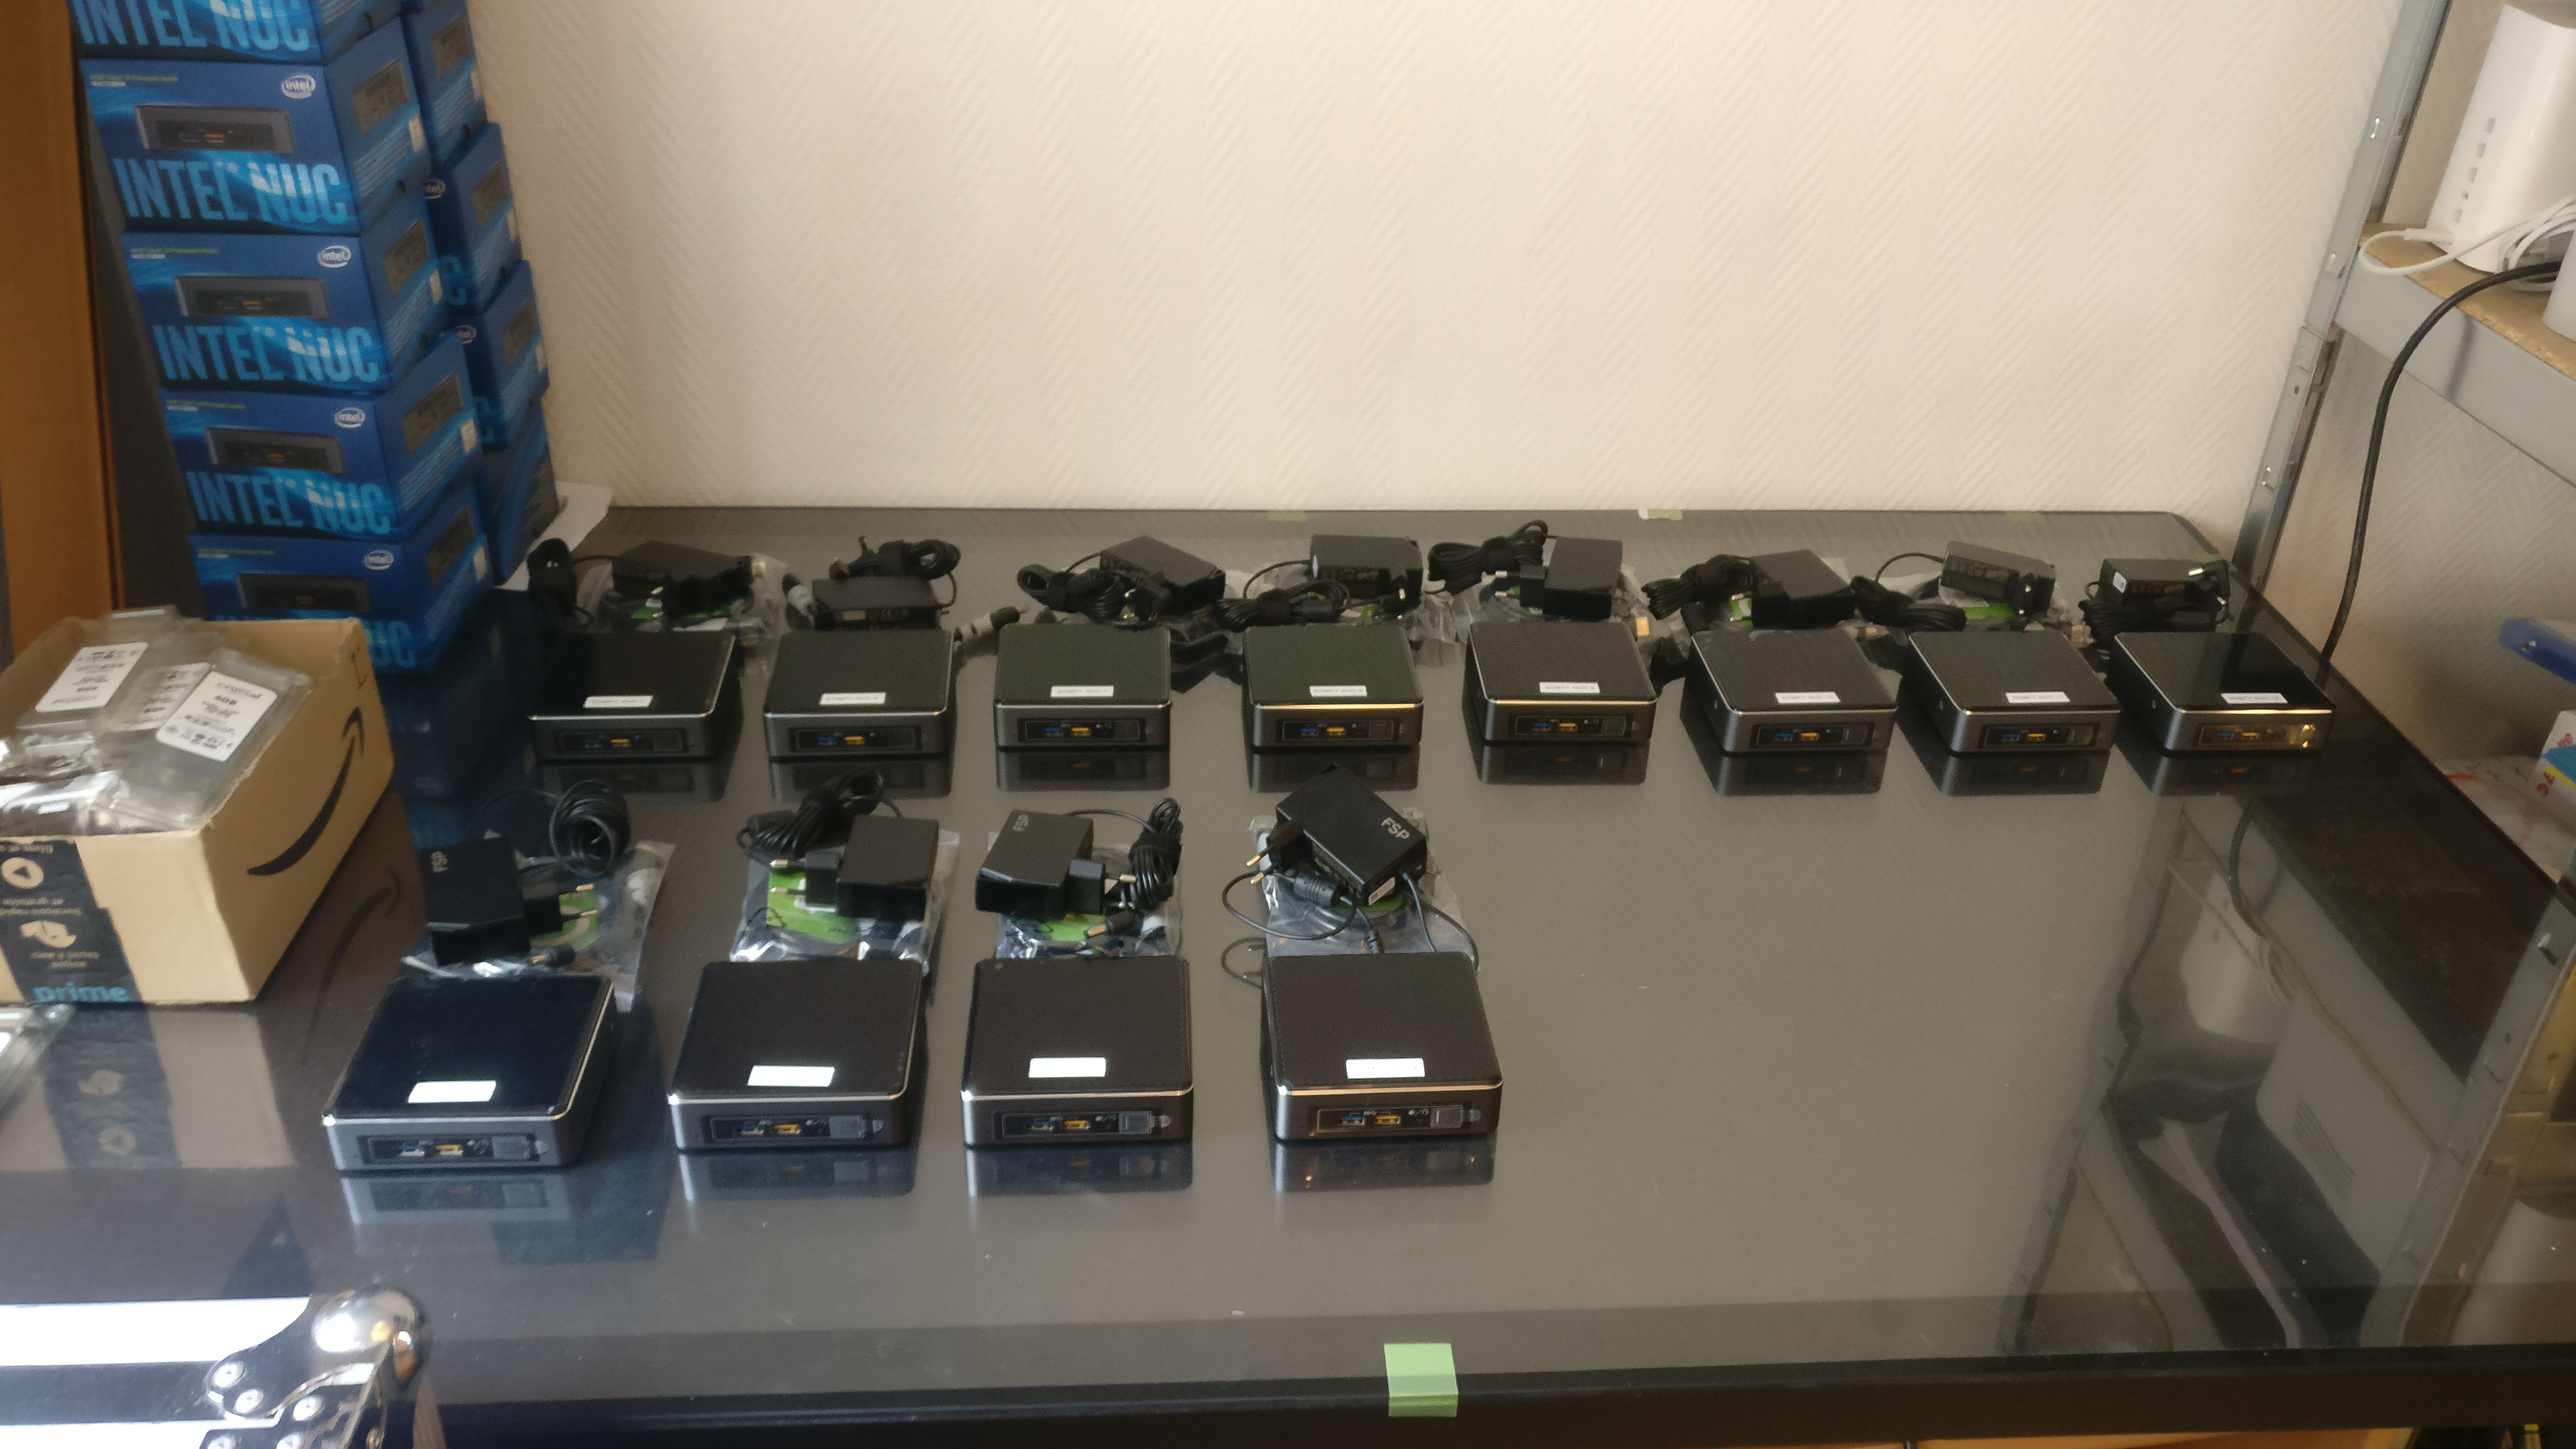
\includegraphics[scale=0.1]{img/somfy-nuc.jpg}
    \caption{Les 12 NUC hebergeant l'application de présentation}
\end{figure}

J'ai donc installé le système sur une machine que l'on apellera master.
J'ai ensuite utilisé CloneZilla pour faire une image du disque de cette machine et pouvoir la répliquer.

Apres l'installation, nous avons trouvé quelques problèmes qui devaient être corrigés.
N'ayant pas le temps de réinstaller un clone sur toutes les machines, nous avons mis en réseau toutes les machines.
Il suffit alors d'utiliser \texttt{cssh} pour éfféctuer les mêmes actions en sychronisé sur toutes les machines.
\texttt{cssh} est un utilitaire permettant de créer un certain nombre de terminaux ssh tous synchronisés;
Il est alors aisé d'administrer un ensemble de machines en même temps.

\begin{figure}[h]
    \centering
    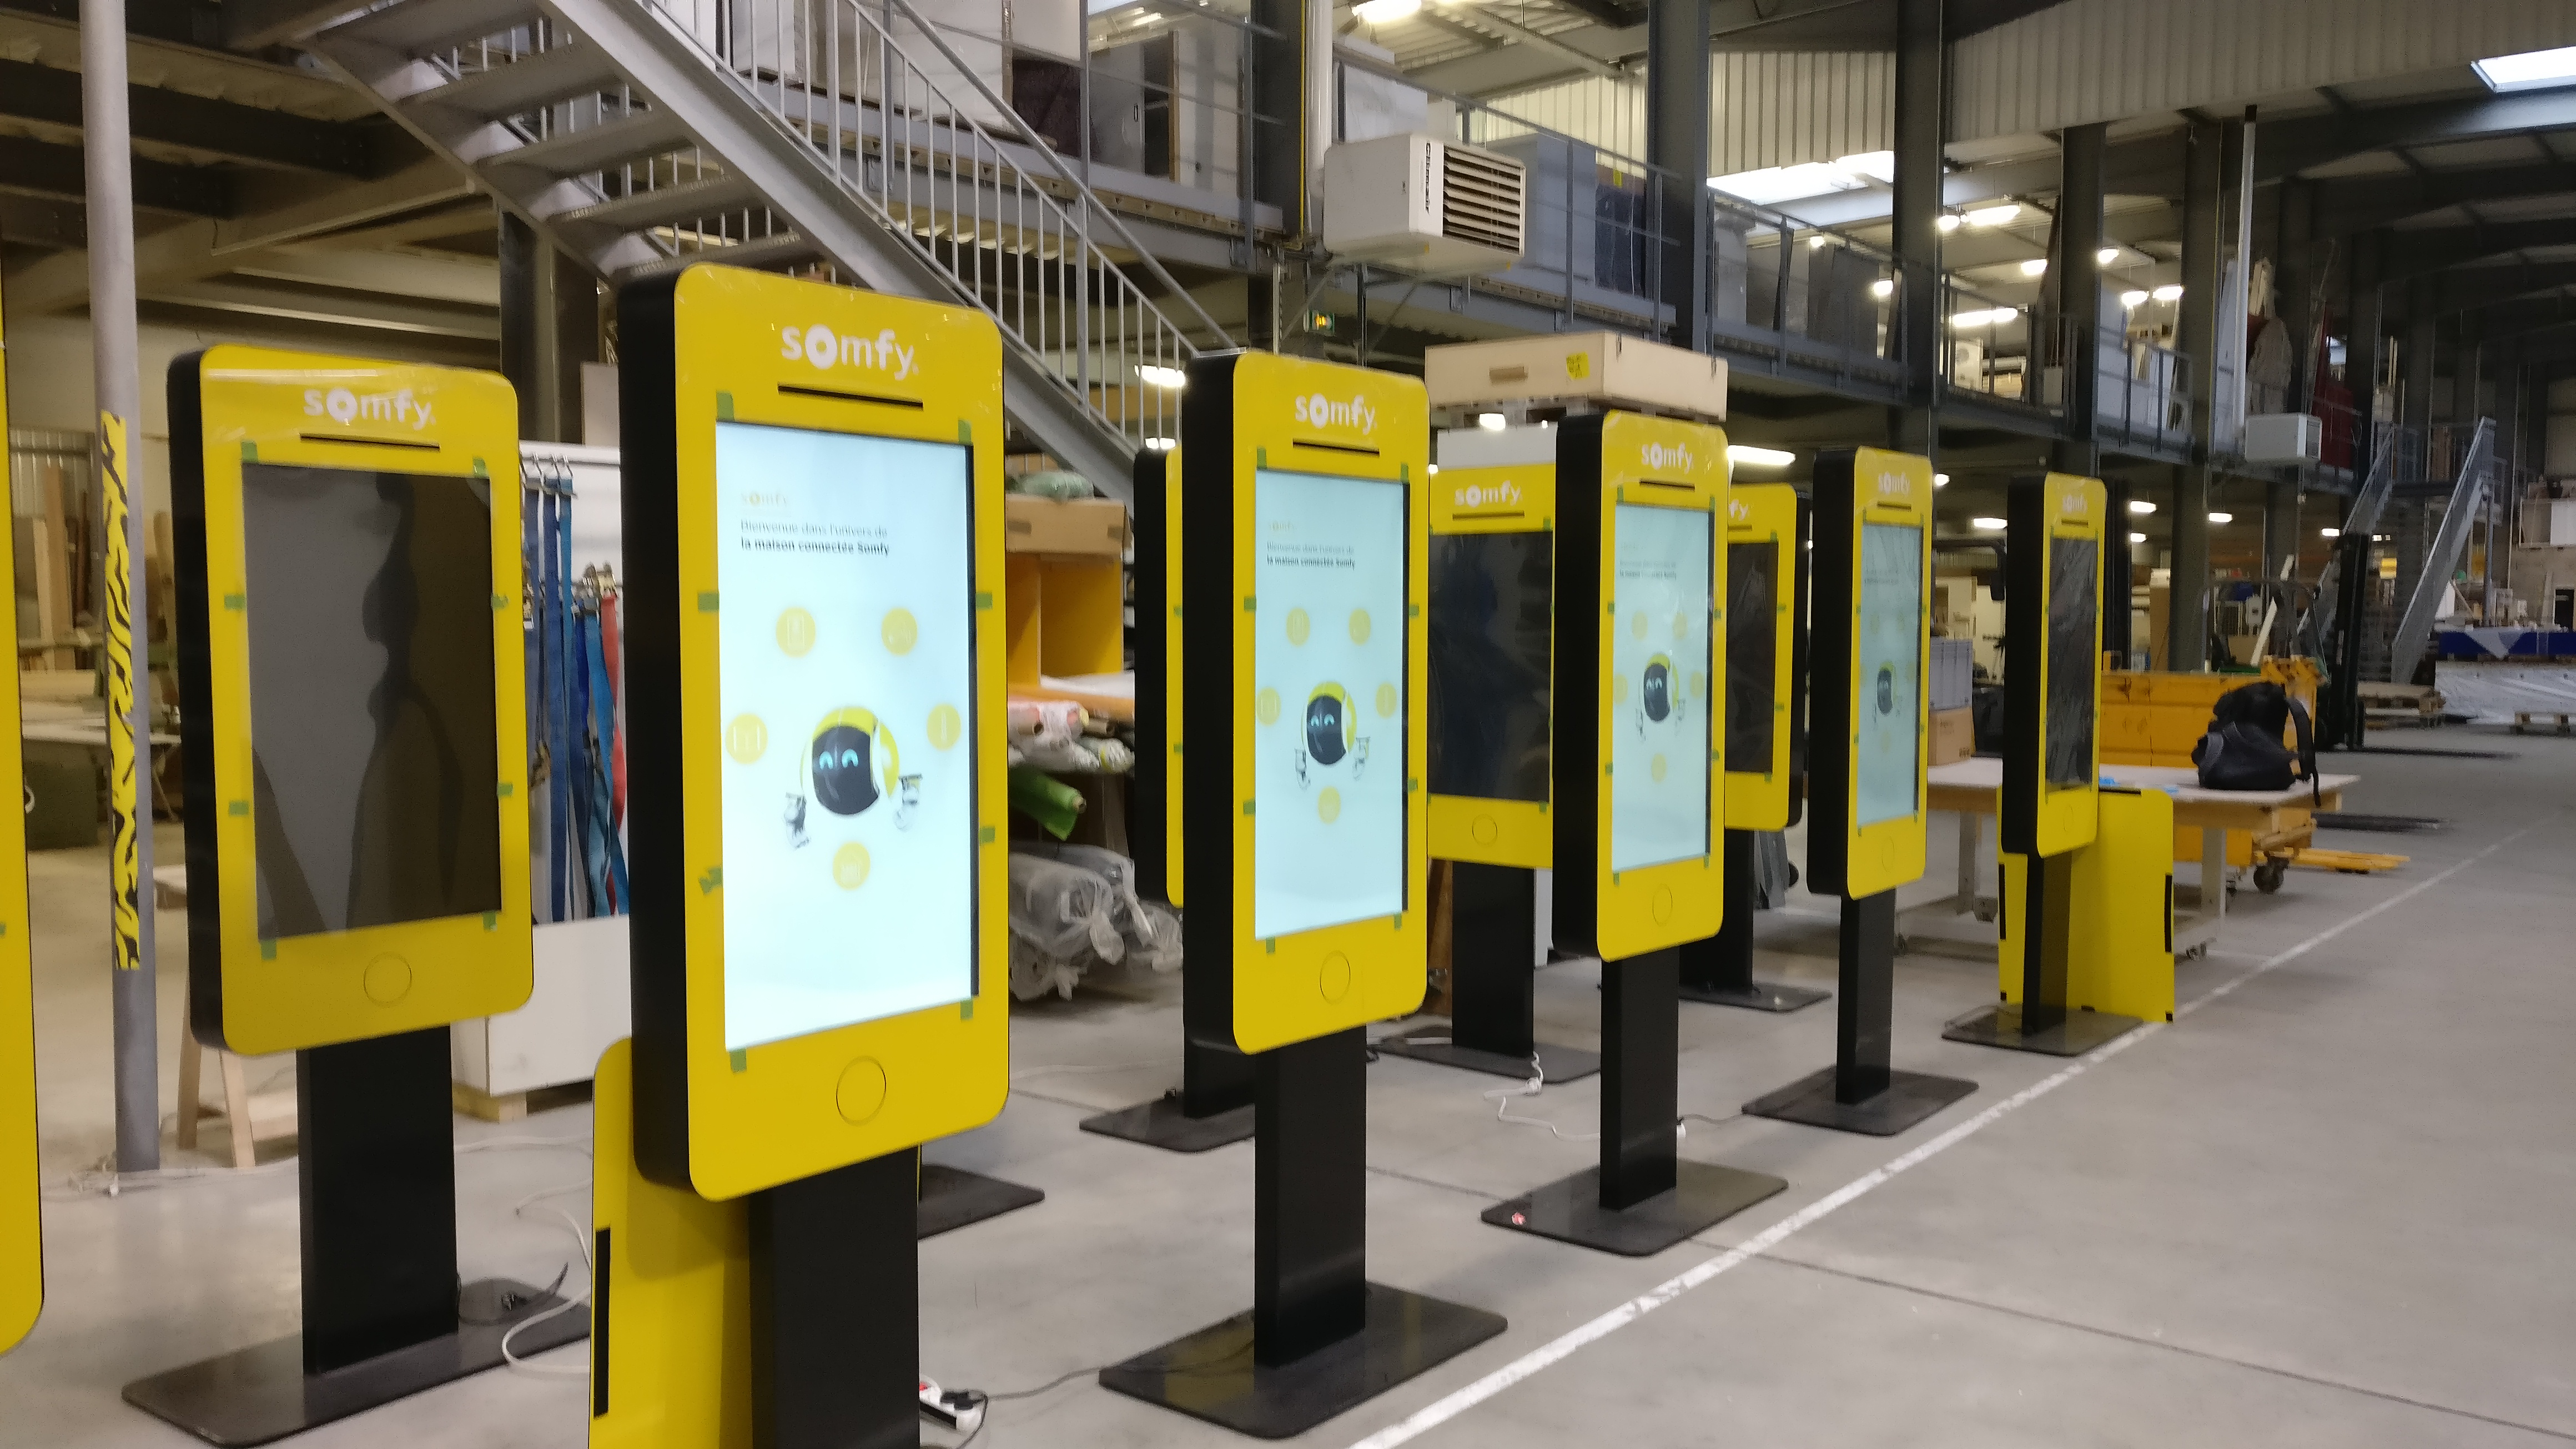
\includegraphics[scale=0.1]{img/somfy-install.jpg}
    \caption{Bornes Somfy lors de l'installation des machines dans leurs abitacles}
\end{figure}

\subsection{Conclusion}

Ce projet fut interessant car il m'a permis de me plonger plus en profondeur sur les composants d'un système linux pour controler son focntionnement.
Malgré la grande partie de recherche pour dégager la meilleur solution, j'ai quand mee eu l'occasion de travailler surn un système de mise à jour innovant.
Le projet est à présent terminé et les bornes ont été disposés dans les magasins vendant la technologie Somfy.

    \section{Media Reader Eiffage}

    \section{Table plan Eiffage}

    \section{Biopedia BioMérieux}

    \section{Bilan}

    \section{Conclusion}

\end{document}
